\documentclass{beamer}

\usepackage{amsmath,amsthm, amssymb, latexsym}

\newcommand{\ts}{\textsuperscript}

% Theme stuff
\usetheme{Madrid}
\useinnertheme{circles}

% Define colors
\definecolor{color0}{RGB}{0,0,0} % black, for text
\definecolor{color1}{RGB}{128,0,0} % maroon, for titles, blocks
\definecolor{color2}{RGB}{118,118,118} % dark grey, for blocks
\definecolor{color3}{RGB}{255,253,250} % background color, white
\definecolor{color4}{RGB}{214,214,206} % light grey, title backgrounds
% Set colors for basic beamer elements
\setbeamercolor{headline}{bg=color4}
\setbeamercolor{footline}{bg=color4}
\setbeamercolor{block title}{bg=color4,fg=color1}
\setbeamercolor{frametitle}{bg=color4,fg=color1}
\setbeamercolor{title}{bg=color4,fg=color1}

\title[quant gen fun]{Some stuff regarding quantitative genetics from a coalescent perspective} 
\author{Evan Koch, Joe Marcus} 
\date{November 3, 2016}

\begin{document}
\frame{\titlepage}
\frame{\tableofcontents}

\section{Introduction}

\begin{frame}{$\mathbf{Q_{ST}}$}
  \framesubtitle{Whitlock, 1999}
  \begin{equation*}
    Q_{ST} = \frac{V_{among}}{V_{among} + 2V_{within}}
  \end{equation*}
  \begin{equation*}
    F_{ST} = \frac{t_{species} - t_{within}}{t_{species}}
  \end{equation*}
    \begin{itemize}
  \item $Q_{ST}$ is a commonly used statistic to test for excessive (or exessively
    uniform) phenotypic differentiation among populations.
  \item Showed that the expectations of $Q_{ST}$ and $F_{ST}$ are equal
  \item Didn't really make that much sense
  \end{itemize}
\end{frame}

\begin{frame}{Schraiber and Landis approach}
  Schraiber and Landis (2015) developed a rigorous coalescent approach to
  studying the sampling distribution of quantitative traits based on the
  coalescent.
  \begin{figure}
    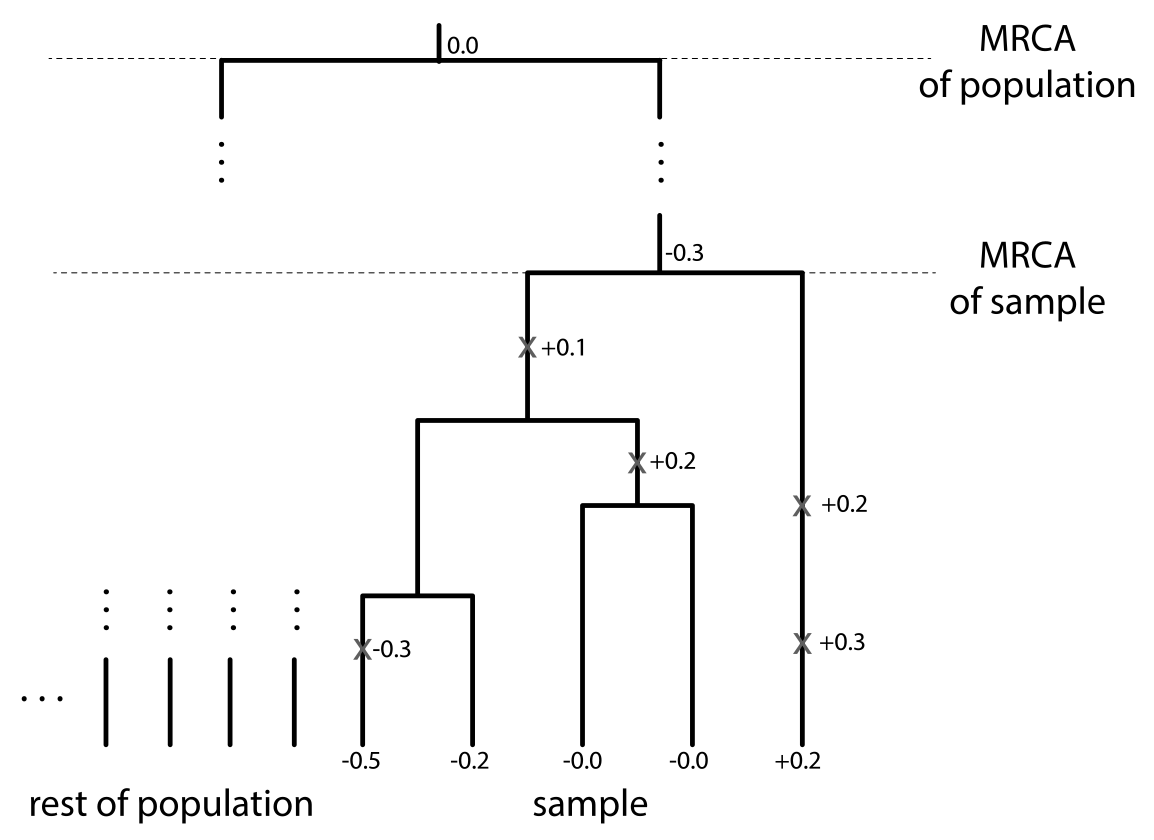
\includegraphics[width=.6\textwidth]{SL.png}
  \end{figure}
\end{frame}

\begin{frame}{Schraiber and Landis approach}
  \begin{itemize}
  \item Main result is a characteristic function for the sampling distribution
    of a quantitative trait under the standard coalescent model for an arbitrary
    stepping stone mutational model.
  \item Derive expected moments from this
  \item Derive limiting distribution when the mutational effects follow a power
    law
  \end{itemize}
\end{frame}

\begin{frame}{Generating functions for coalescent models have been examiend in some detail}
  \framesubtitle{Lohse, Harrison, and Barton (2011)}
  Derive generating functions for 
  \begin{itemize}
  \item Structured coalescent
  \item Rate changes
  \item Linked loci
  \end{itemize}
\end{frame}

\section{Mathematical results}
\subsection{A general moment generating function}
\begin{frame}{Extending Schraiber and Landis (2015) results to aribitary
    genealogical distributions}
  \begin{itemize}
  \item[$\mathbf{T}$] : random vector containing lengths of all possible
    branches in the genealogy \\(ex:
    $\mathbf{T}=\{T_a,T_b,T_c,T_{a,b},T_{a,c},T_{b,c}\}$).
  \item[$\mathcal{O}$] : all possible configurations that coalescent branches
    can subtend\\ (ex: $\mathcal{O}=\{\{a\},\{b\},\{c\},\{a,b\},\{a,c\},\{b,c\}\}$).
  \item[$\mathbf{Y}$] : quantitative trait 'values' in the sampled individuals\\
    (ex: $\mathbf{Y}=\{Y_a,Y_b,Y_c\}$).
  \end{itemize}
\end{frame}

\begin{frame}{The moment generating function for trait values}
  \begin{equation*}
    \varphi_{\mathbf{Y}}(\mathbf{k}) = E\left[ e^{\mathbf{k} \cdot \mathbf{Y}} \right] =
    \int e^{\mathbf{k} \cdot \mathbf{Y}} P(\mathbf{Y}=\mathbf{y}) d\mathbf{y},
  \end{equation*}
  $k$ is a vector a dummy variables for each sample. \\
  Conditioning on the genealogy...
  \begin{align}
    \varphi_{\mathbf{Y}}(\mathbf{k}) &= \int e^{\mathbf{k} \cdot \mathbf{Y}}
    \int P(\mathbf{Y}=\mathbf{y} | \mathbf{T}=\mathbf{t})
    P(\mathbf{T}=\mathbf{t}) d\mathbf{t} d\mathbf{y}\\ &= \int \int
    e^{\mathbf{k} \cdot \mathbf{Y}} P(\mathbf{Y}=\mathbf{y} |
    \mathbf{T}=\mathbf{t}) d\mathbf{y} P(\mathbf{T}=\mathbf{t}) d\mathbf{t}
  \end{align}
\end{frame}

\begin{frame}{Splitting trait change across branches}
  \begin{equation*}
    Y_i = \sum_{\omega \in \mathcal{O}} Y_{i,\omega}
  \end{equation*}
  $Y_{i,\omega}$ are conditionally independent given $\mathbf{T}$. 
  \begin{equation*}
    \mathbf{k} \cdot \mathbf{y} = \sum_{\omega \in \mathcal{O}}\left( \sum_{i \in \omega} k_iy_{i,\omega}\right)
  \end{equation*}
  \begin{equation*}
    P(\mathbf{Y}=\mathbf{y}|\mathbf{T}=\mathbf{t}) = \prod_{\omega \in \mathcal{O}}
    P(\mathbf{Y}_{\omega}=(y_{i,\omega})_{i \in \omega} | \mathbf{T}=\mathbf{t}).
  \end{equation*}
  \footnotesize
  \begin{equation*} \label{eq:factor}
    \int e^{\mathbf{k} \cdot \mathbf{Y}} P(\mathbf{Y}=\mathbf{y} |\mathbf{T}=\mathbf{t}) d\mathbf{y} =
    \prod_{\omega \in \mathcal{O}}\int \exp\left(\sum_{i \in \omega}k_iy_{i,\omega}\right)
    P(\mathbf{Y}_{\omega}=(y_{i,\omega})_{i \in \omega} | \mathbf{T}=\mathbf{t})d(y_{i,\omega})_{i \in \omega}.
  \end{equation*}
  \normalsize
\end{frame}

\begin{frame}{Two important moment generating function facts}
  \begin{block}{mgf of compound poisson process}
    \begin{equation*}
      \exp\left(\lambda t (\psi(k)-1)\right)
    \end{equation*}
    $\lambda$ is the rate that events occur and $\psi$ is the distribution that
    the effects of events are drawn from. 
  \end{block}
  \begin{block}{mgf of completely correlated random variables}
    If $X_1=X_2$ then the mgf of their joint distribution is
    $\varphi_{X_1}(k_1+k_2)$.\\
    This is relevant because the effects of mutations along branches are shared
    by all descendants.
  \end{block}
\end{frame}

\begin{frame}{The mgf for a general distribution of genealogies}
  \begin{equation*}
    \varphi_{\mathbf{Y}}(\mathbf{k}) = \prod_{\omega \in \mathcal{O}}
    \int \exp\left( \frac{\theta}{2} t_{\omega} \left( \psi\left(\sum_{a \in \omega}k_{a}\right) -1 \right)\right)
    P(\mathbf{T}=\mathbf{t})d\mathbf{t}.
  \end{equation*}
  This is simply the moment generating function for the genealogy
  $\mathbf{T}$ with $\frac{\theta}{2} \left( \psi(\sum_{i \in
      \omega}k_{\omega}) -1 \right)$ substituted for the dummy variable of
  branch $T_{\omega}$. Or,
  \begin{equation*}
    \label{eq:sub}
    \varphi_{\mathbf{T}}(\mathbf{s})\Bigr|_{s_{\omega}=\frac{\theta}{2} \left( \psi\left(\sum_{a \in \omega}k_{a}\right) -1 \right)}
  \end{equation*}
  Would multiply by $L$ to get a trait affected by $L$ different loci.
\end{frame}

\subsection{Connection to previous results}

\begin{frame}{Schraiber and Landis + Lohse et al.}
  \begin{block}{Lohse et al. 2011}
    \begin{equation*}
      \varphi_{T}\left( \mathbf{s} \right) = \frac{
        \sum_i \lambda_i \varphi_i(\mathbf{s})}{
        \sum_i \lambda_i - \sum_{|\omega|=1}s_{\omega}}.
    \end{equation*}
  \end{block}
  \begin{block}{Schraiber and Landis 2015}
    \begin{equation*}
      \varphi_{Y}\left( \mathbf{k} \right) = \frac{2}{
        n(n-1) - \theta \left( \sum_{u=1}^n \psi(k_u) - n\right)} \sum_{u<v}\varphi_{n-1}(\mathbf{k}^{(u,v)})
    \end{equation*}
  \end{block}
  Can obtain 2nd result from substitution into the first.
\end{frame}

\begin{frame}{An example in structured populations}
  \begin{align}
    \varphi_{\mathbf{T}}^{\Omega}(\mathbf{s}) &= \left( \sum_{i=1}^M
    \binom{|\Omega_i|}{2}\eta_i + \sum_{(i,j:i \neq j)} m_{i,j}|\Omega_i| -
    \sum_{i=1}^M \sum_{\omega \in \Omega_i}s_{\omega}\right)^{-1} \nonumber
    \\ &\times \left( \sum_{i=1}^M \eta_i \sum_{(a,b) \in \Omega_i:a \neq b}
    \varphi_{\mathbf{T}}^{\Omega(i:a \cup b)}(\mathbf{s}) + \sum_{(i,j):i\neq
      j}m_{i,j}\sum_{\omega \in \Omega_i} \varphi_{\mathbf{T}}^{\Omega\left( i
      :-\omega, j: + \omega \right)}(\mathbf{s})\right). \nonumber
  \end{align}
\end{frame}

\subsection{A central limit theorem to get the infinitesimal model}

\begin{frame}{Central limit theorem}
  \begin{equation*}
    \varphi_T(\mathbf{s}) = \int \exp \left( \sum_{\omega \in \mathcal{O}} s_{\omega}t_{\omega} \right)
    P(\mathbf{T}=\mathbf{t})d\mathbf{t}. \nonumber
  \end{equation*}
  Taking a Taylor series we get
  \scriptsize
  \begin{align}
    \label{eq:mgf_L}
    &\left(\int \exp \left( \sum_{\omega \in \mathcal{O}} s_{\omega}t_{\omega}
      \right)P(\mathbf{T}=\mathbf{t})d\mathbf{t}\right)^L = \nonumber \\  &\left(1 + \sum_{\omega \in \mathcal{O}}
      s_{\omega}E[t_{\omega}] + \sum_{\omega_1 \neq \omega_2}
      s_{\omega_1}s_{\omega_2}E[t_{\omega_2}t_{\omega_1}] + \sum_{\omega \in
        \mathcal{O}} \frac{s_{\omega}^2E[t_{\omega}^2]}{2} + \ldots\right)^L. \nonumber
  \end{align}
  \normalsize
\end{frame}

\begin{frame}{Central limit theorem}
  Also taking the Taylor series of $\psi$ and making the appropriate substitution we get
  \begin{equation*}
    \left( 1 + \frac{\theta}{2} \sum_{\omega \in \mathcal{O}} E[t_{\omega}]\left( m \left(
          \sum_{a \in \omega} k_a\right) + \frac{\tau^2}{2}\left( \sum_{a \in \omega}
          k_a\right)^2 + \ldots\right)\right)^L.
  \end{equation*}
  Taking the limit such that $Lm \to \mu$ and $L\tau^2\to \sigma^2$ as $L
  \to \infty$ we get
  \begin{equation*}
    \exp \left( \frac{\theta}{2} \sum_{\omega \in \mathcal{O}}E[t_{\omega}] \left( \mu \left(
          \sum_{a \in \omega} k_a\right) + \frac{\sigma^2}{2}\left( \sum_{a \in \omega}
          k_a\right)^2\right)\right),
  \end{equation*}
\end{frame}

\begin{frame}{Central limit theorem}
  $Y$ is multivariate normal with 
  \begin{equation*}
    E[Y_i] = \frac{\theta}{2} E[T_{MRCA}] \mu
  \end{equation*}
  \begin{equation*}
    Var[Y_i] = \frac{\theta}{2} E[T_{MRCA}] \sigma^2
  \end{equation*}
  \begin{equation*}
    Cov[Y_i, Y_j] = \frac{\theta}{2} (T_{MRCA}-E[\mathfrak{t}_{1,2}] )\sigma^2
  \end{equation*}
\end{frame}

\begin{frame}{The distribution of individual differences}
  \small
  \begin{equation*}
    \label{eq:cov}
    Cov[Y_1-Y_2,Y_3-Y_4]=Cov[Y_1,Y_3]+Cov[Y_2,Y_4]-Cov[Y_1,Y_4]-Cov[Y_2,Y_3]
  \end{equation*}
  \begin{equation*}
    \label{eq:covcoal}
    Cov[Y_1-Y_2,Y_3-Y_4] \propto E[\mathfrak{t}_{1,4}] + E[\mathfrak{t}_{2,3}] - E[\mathfrak{t}_{1,3}] - E[\mathfrak{t}_{2,4}].
  \end{equation*}
\end{frame}

\section{Futher research}
\subsection{Is this just trivial?}

\begin{frame}{Is this just trivial?}
  maybe?
\end{frame}

\subsection{Alternate mutational distributions}

\begin{frame}{Other potential mutational distributions}
  \begin{block}{Random walk mutation model (Crow and Kimura, 1964)}
    \begin{equation*}
      u(x,y) = u_{RW}(y-x)
    \end{equation*}
  \end{block}
  \begin{block}{House-of-cards mutation model (Kingman 1979)}    
    \begin{equation*}
      u(x,y) = u_{HC}(y)
    \end{equation*}
  \end{block}
  \begin{block}{Zeng and Cockerham (1993)}    
    \begin{equation*}
      u(x,y) = u_{ZC}(y - cx)
    \end{equation*}
  \end{block}
  These destroy the compound Poisson process portion of things.
\end{frame}

\subsection{The distribution of quantitative traits in structured populations}

\end{document}
